\newsavebox{\articles}
\sbox{\articles}{
    \begin{tikzpicture}
        \begin{axis}[
            height=6cm,
            width=9cm,
            xmin=1990,
            xmax=2024,
            xtick={1990, 1995, 2000, 2005, 2010, 2015, 2020},
            xticklabels={1990, 1995, 2000, 2005, 2010, 2015, 2020},
            xlabel={Year},
            ymin=0,
            ymax=8000,
            ytick={2000, 4000, 6000},
            yticklabels={2000, 4000, 6000},
            ylabel={Number of publications},
            ylabel style={align=center, font=\small\linespread{0.9}\selectfont, yshift=0.4cm},
            xlabel style={font=\small},
            xtick pos=bottom,
            ytick pos=left,
            ticklabel style={font=\small},
            axis lines=left,
            clip=false
        ]
            \addplot[
                cyan,
                very thick,
                stealth-
            ] table[
                col sep=comma,
                x=Year,
                y=Count
            ] {data/PubMed_Timeline_Results_by_Year.csv};
        \end{axis}
    \end{tikzpicture}
}

\begin{frame}{Do we need explainable AI?}
    \begin{tikzpicture}
        \node[] at (-5.25, 3.5) {};
        \node[] at (5.25, -3.5) {};

        \only<1>{
            \node[inner sep=0pt, draw=black] at (0, 0) {
                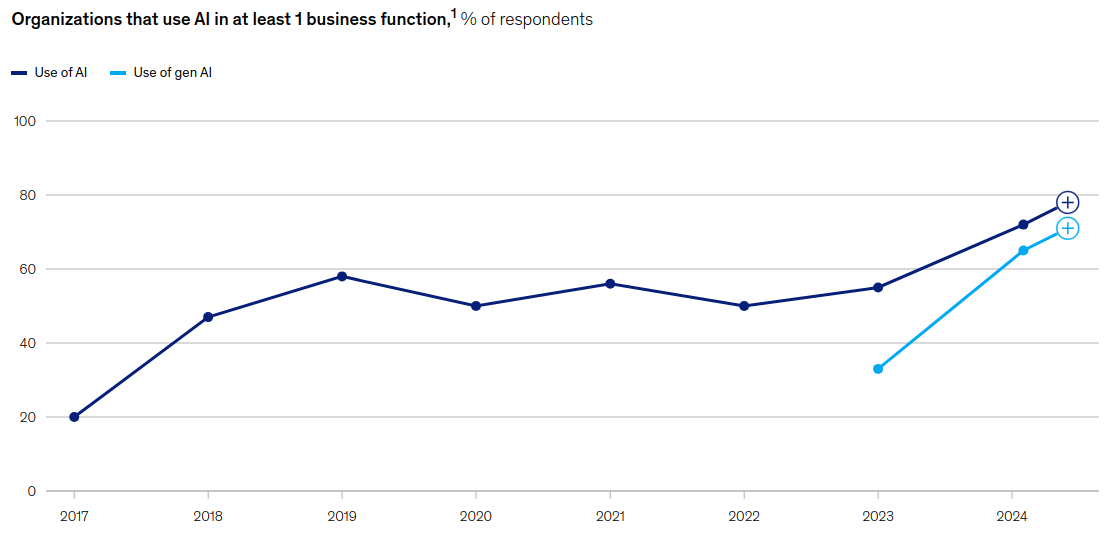
\includegraphics[width=10cm]{data/mckinsey.png}
            };
            \node[anchor=south, font=\tiny, text width=10.5cm, align=flush center] at (0, -3.75) {
                McKinsey \& Company, The state of AI: How organizations are rewiring to capture value, \textit{\url{https://www.mckinsey.com/capabilities/quantumblack/our-insights/the-state-of-ai}} (2025)
            };
        }
        \only<2>{
            \node[] at (0, 0) {
                \usebox{\articles}
            };
            \node[anchor=south, font=\tiny, text width=10.5cm, align=flush center] at (0, -3.75) {
                Publications from \url{https://pubmed.ncbi.nlm.nih.gov/} containing "(neurology OR neuroscience OR neuroimaging) AND (ai OR artificial intelligence OR deep learning)"
            };
        }
        \only<3>{
            \node[] at (0, 0) {AI in norwegian health care};
        }
        \only<4>{
            \node[] at (0, 0) {AI medicine ethics};
        }
        \only<5>{
            \node[] at (0, 0) {Medical practitioner statistics};
        }
    \end{tikzpicture}
\end{frame}

\begin{frame}{What is explainable AI?}
    \newcommand{\neuron}[3]{
        \node[circle, draw=black, fill=####2] (####1) at ####3 {};
    }

    \def\hsep{0.7}
    \def\vsep{0.5}
    \def\edgecolor{gray}
    \def\edgeopacity{0.5}
    \def\neuroncolour{gray}

    \begin{tikzpicture}

        \node[] at (-5.25, -3.25) {};
        \node[] at (5.25, 3.25) {};

        \node[
            draw=black,
            fill=babalightblue!50,
            minimum height=2.8cm,
            minimum width=4.3cm
        ] (model) at (0, 1) {};
        \node[
            anchor=south,
            font=\small
        ] at (model.north) {Artificial neural network};

        \neuron{n00}{\neuroncolour}{($ (model) + (-2 * \hsep, -2 * \vsep) $)}
        \neuron{n01}{\neuroncolour}{($ (model) + (-2 * \hsep, -\vsep) $)}
        \neuron{n02}{\neuroncolour}{($ (model) + (-2 * \hsep, 0) $)}
        \neuron{n03}{\neuroncolour}{($ (model) + (-2 * \hsep, \vsep) $)}
        \neuron{n04}{\neuroncolour}{($ (model) + (-2 * \hsep, 2 * \vsep) $)}

        \neuron{n10}{\neuroncolour}{($ (model) + (-\hsep, -1.5 * \vsep) $)}
        \neuron{n11}{\neuroncolour}{($ (model) + (-\hsep, -0.5 * \vsep) $)}
        \neuron{n12}{\neuroncolour}{($ (model) + (-\hsep, 0.5 * \vsep) $)}
        \neuron{n13}{\neuroncolour}{($ (model) + (-\hsep, 1.5 * \vsep) $)}

        \neuron{n20}{\neuroncolour}{($ (model) + (0, -\vsep) $)}
        \neuron{n21}{\neuroncolour}{(model)}
        \neuron{n22}{\neuroncolour}{($ (model) + (0, \vsep) $)}

        \neuron{n30}{\neuroncolour}{($ (model) + (\hsep, -0.5 * \vsep) $)}
        \neuron{n31}{\neuroncolour}{($ (model) + (\hsep, 0.5 * \vsep) $)}

        \neuron{n40}{\neuroncolour}{($ (model) + (2 * \hsep, 0) $)}

        \draw[-stealth, \edgecolor, opacity=\edgeopacity] (model.west) -- (n00);
        \draw[-stealth, \edgecolor, opacity=\edgeopacity] (model.west) -- (n01);
        \draw[-stealth, \edgecolor, opacity=\edgeopacity] (model.west) -- (n02);
        \draw[-stealth, \edgecolor, opacity=\edgeopacity] (model.west) -- (n03);
        \draw[-stealth, \edgecolor, opacity=\edgeopacity] (model.west) -- (n04);


    \end{tikzpicture}
\end{frame}